\documentclass{beamer}

\usepackage{mathtools}
\usepackage{hyperref}
\usepackage{physics}
\usepackage{graphicx}
\usepackage{float}
\usepackage{subfigure}
\usepackage{color}
\usepackage{cite}
\usepackage[numbers]{gbt7714}
\usepackage{indentfirst}
\setlength{\parindent}{2em}
\usepackage{pifont}
\usepackage{comment}
\usepackage[orientation=landscape,size=custom,width=16,
height=9,scale=0.5,debug]{beamerposter}
\usepackage{wrapfig}
\hypersetup{pdfpagemode=FullScreen}
\usepackage{multicol}
\usepackage{amsmath,amssymb}
\usepackage{fontspec}
\usepackage{unicode-math}
\usepackage{listings}
\usepackage{algorithm}

\setmainfont{Times New Roman}
\setmathfont{XITS Math}


\title{Simulations with MPS}
\author{Kunyang DU}
\institute{Institue of Theoretical Physics}
\date{\today}

\begin{document}

\begin{frame}
	\titlepage
\end{frame}

\begin{frame}
	\frametitle{Model}
	\begin{itemize}
		\item \textbf{Hamiltonian:} Transverse Ising Model
		\begin{equation}
			H = J\sum_{i}^{N-1}\sigma_i \sigma_{i+1} + h\sum_i^N\sigma_i
		\end{equation}
		\item \textbf{Parameters} Physics parameters:
		\begin{equation}
			J = 1.0,\quad h = 0.5,\quad N = 12
		\end{equation}
		Numerical parameters:
		\begin{equation}
			d = 2,\quad D_{MPO} = 3, \quad D_{MPS} = 128
		\end{equation}
	\end{itemize}
\end{frame}

\begin{frame}
	\frametitle{DMRG}
	\begin{multicols*}{2}
	\begin{itemize}
		\item Initialize MPS with diagonalization center at $i=1$.
		\begin{figure}[H]
			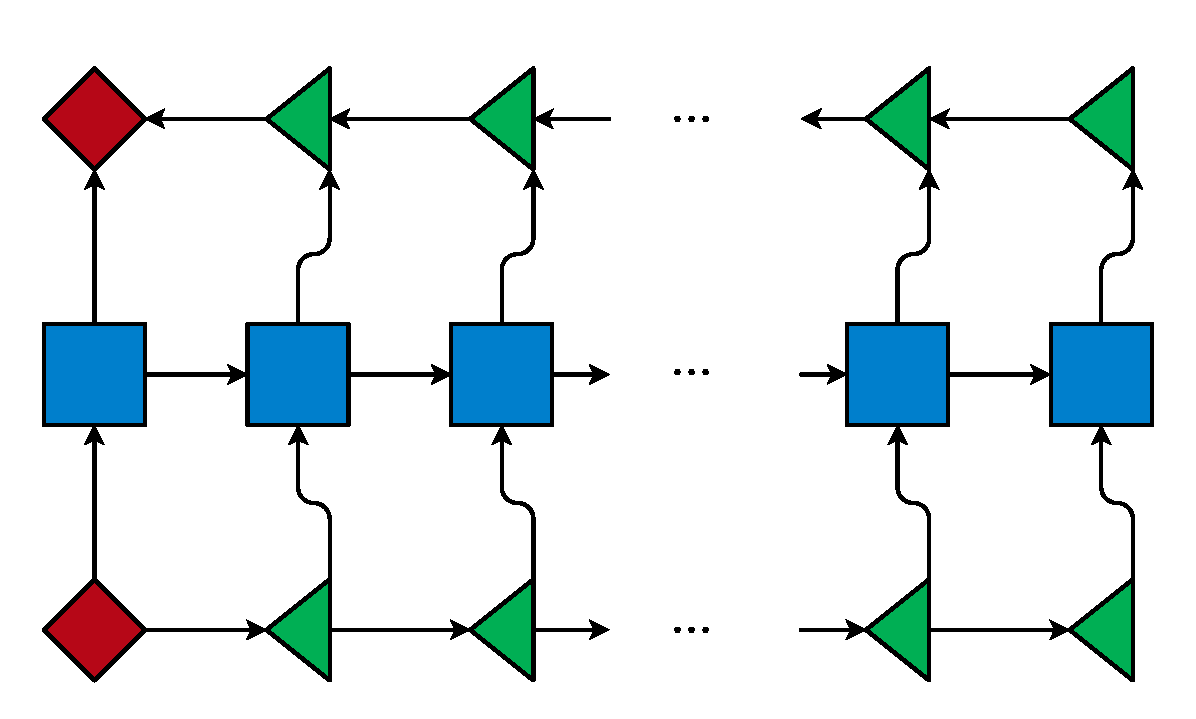
\includegraphics[width=1. \linewidth]{images/Initialization.pdf}
		\end{figure}
		\newpage
		\item Sweep at two direction (right - left - right - \dots)
		\begin{itemize}
			\item Calculate the left/right environment $H_L/H_R$.
			\begin{figure}[H]
				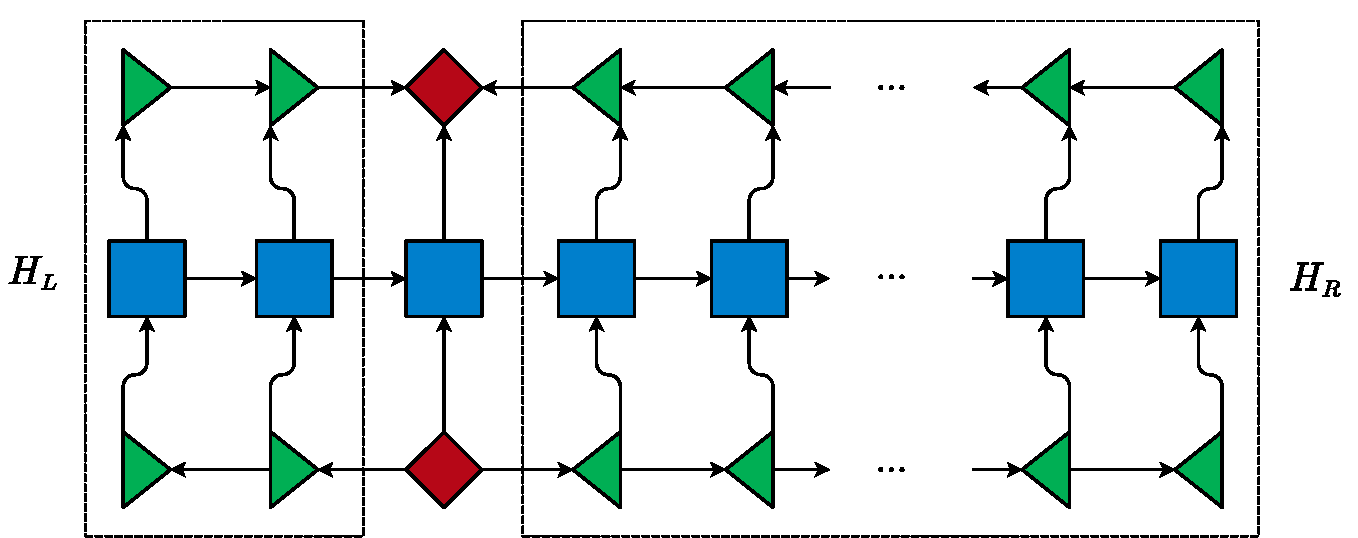
\includegraphics[width=1. \linewidth]{images/LRenv1.pdf}
			\end{figure}
		\end{itemize}
	\end{itemize}
	\end{multicols*}
\end{frame}

\begin{frame}
	\frametitle{DMRG}
	\begin{itemize}
		\item Sweep at two direction (right - left - right - \dots)
		\begin{itemize}
			\item Calculate the effective Hamiltonian $H_{eff} = H_L H_i H_R$
			\begin{figure}[H]
				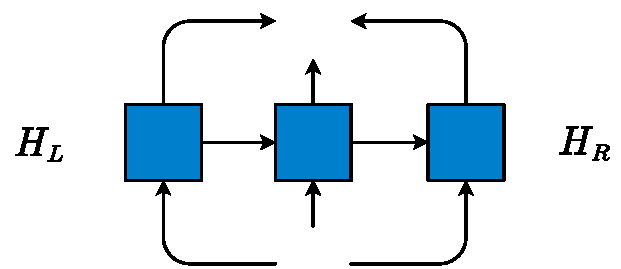
\includegraphics[width=0.3 \linewidth]{images/effH1.pdf}
			\end{figure}
			\item OrientSVD and move the center to next site.
			\begin{figure}[H]
				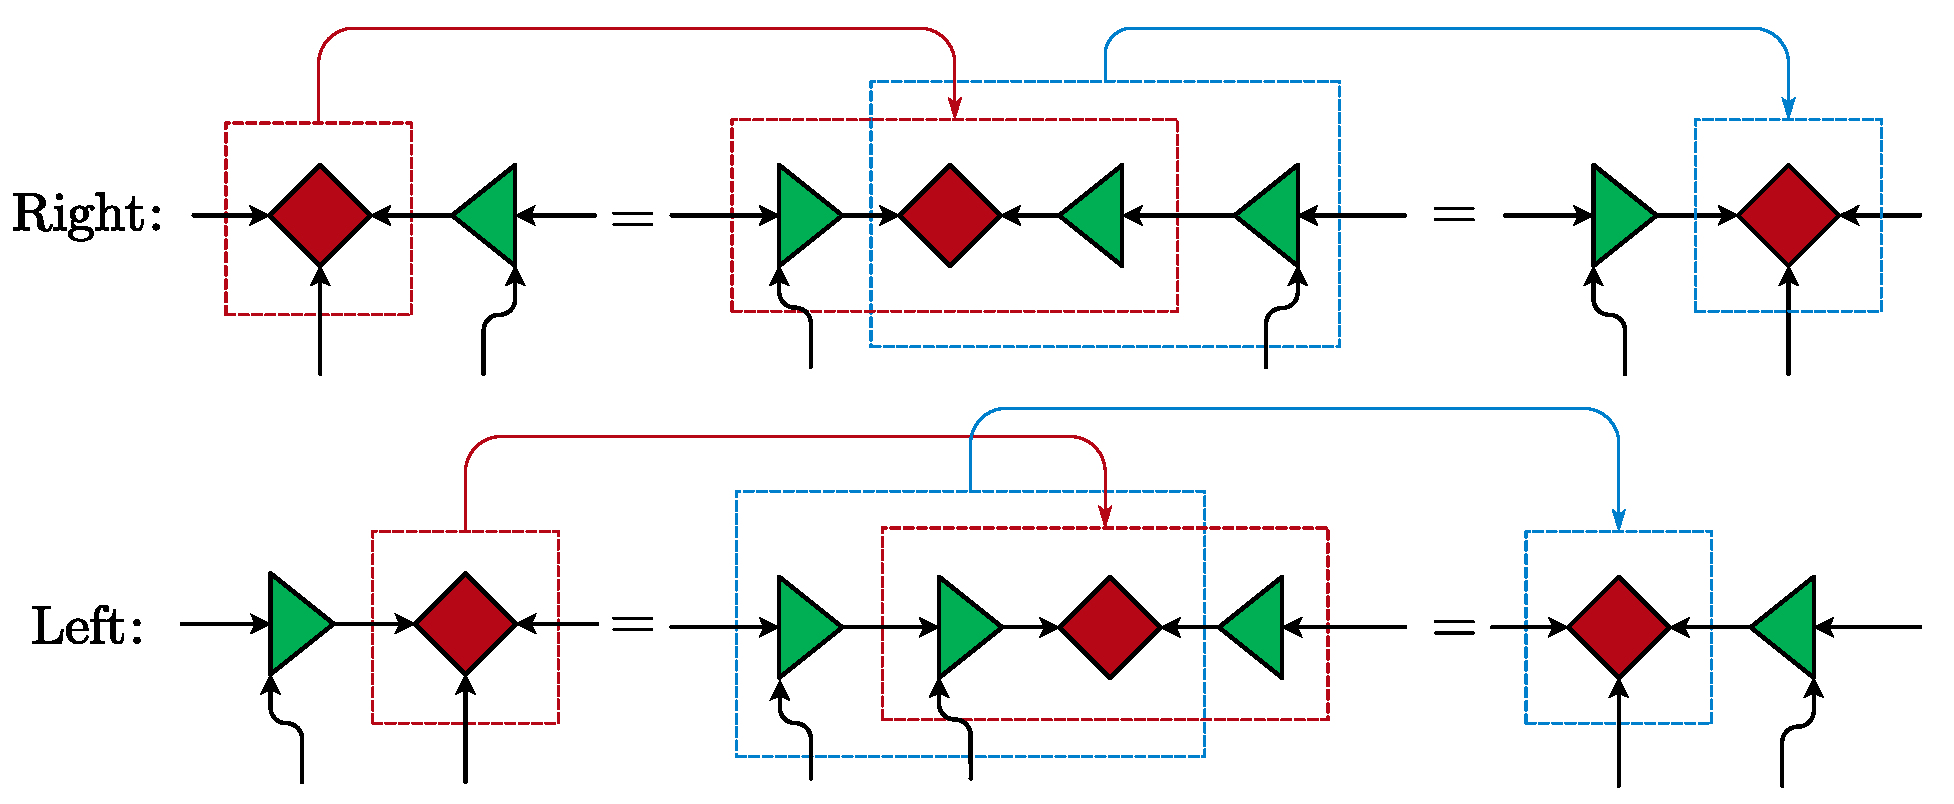
\includegraphics[width=0.6 \linewidth]{images/orientSVD.pdf}
			\end{figure}
		\end{itemize}
	\end{itemize}
\end{frame}


\begin{frame}
	\frametitle{TDVP: 1-site integration}
	\begin{itemize}
		\item Initialize MPS with diagonalization center at $i=1$.
		\newpage
		\item Sweep at two direction (right - left - right - \dots)
		\begin{itemize}
			\item Calculate the left/right environment $H_L(t+\Delta t/2)/H_R(t)$.
			\begin{figure}[H]
				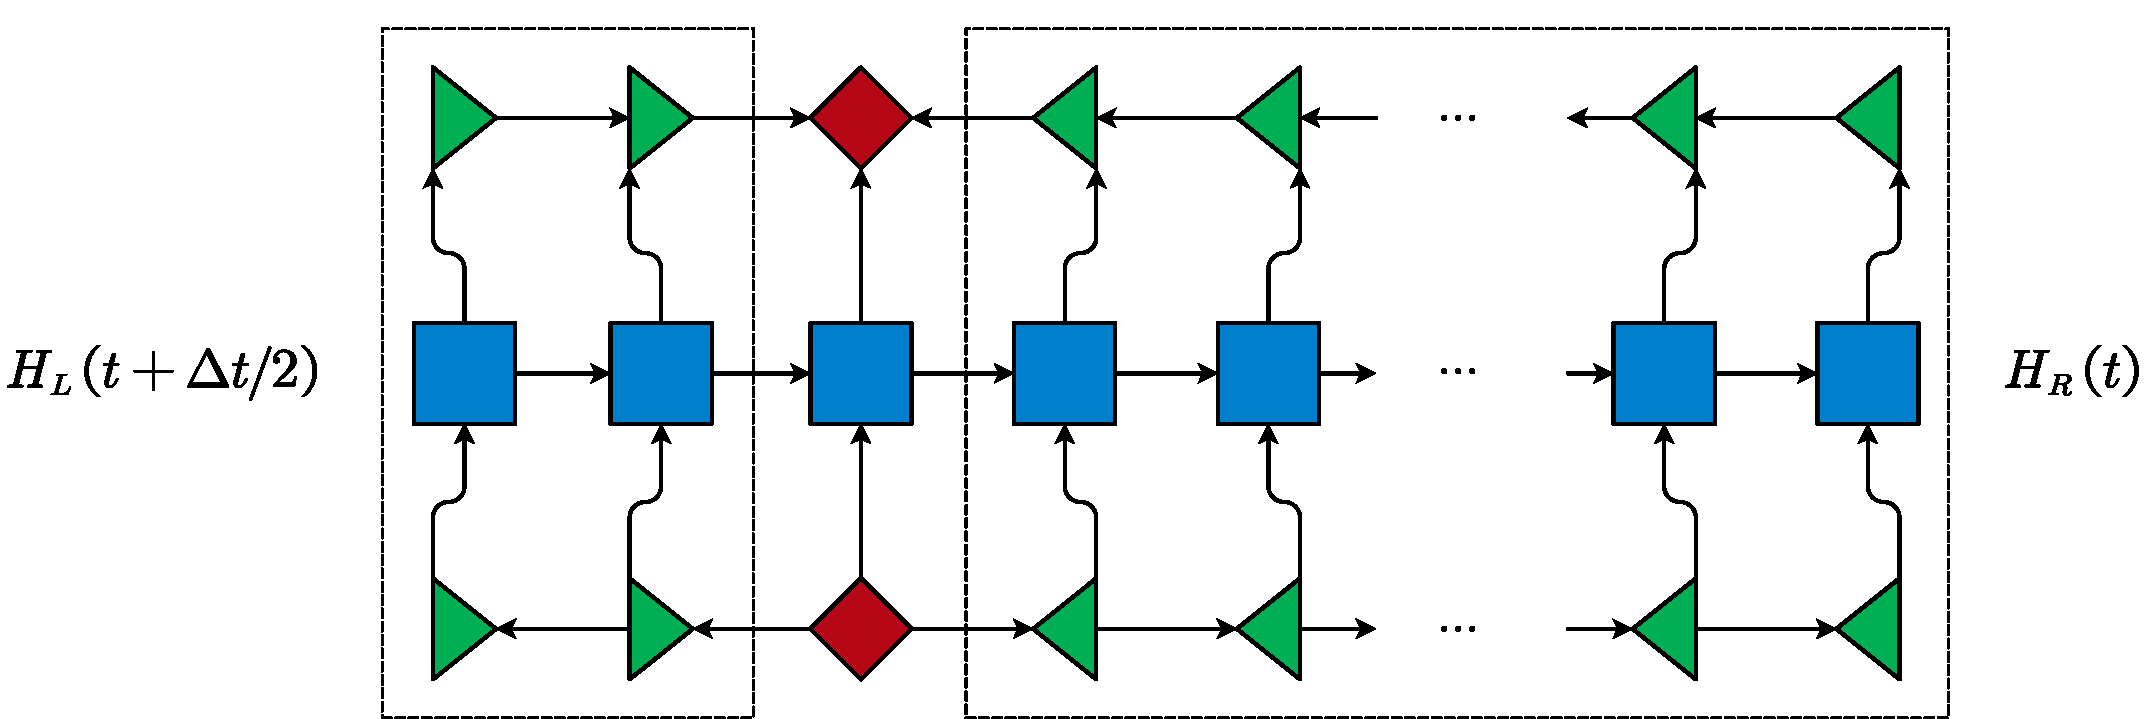
\includegraphics[width=0.8 \linewidth]{images/LRenv1 t.pdf}
			\end{figure}
		\end{itemize}
	\end{itemize}
\end{frame}

\begin{frame}
	\frametitle{TDVP: 1-site integration}
	\begin{itemize}
		\item Sweep at two direction (right - left - right - \dots)
		\begin{itemize}
			\item Calculate the effective Hamiltonian $H_{eff}^{(1)}$
			\item Time evolution $A_i(t+\Delta t/2) = \exp(-iH_{eff}^{(1)}\Delta t / 2)A_i(t)$ 
			\item OrientSVD and calculate the center with inverse evolution $C_i(t) = \exp(iH_{eff}^{(0)}\Delta t /2) C_i(t+\Delta t/2)$, then absorb it into nextsite.
			\setcounter{subfigure}{0}
			\begin{figure}[H]
				\centering
				\subfigbottomskip=2pt
				\subfigcapskip=-5pt
				\subfigure{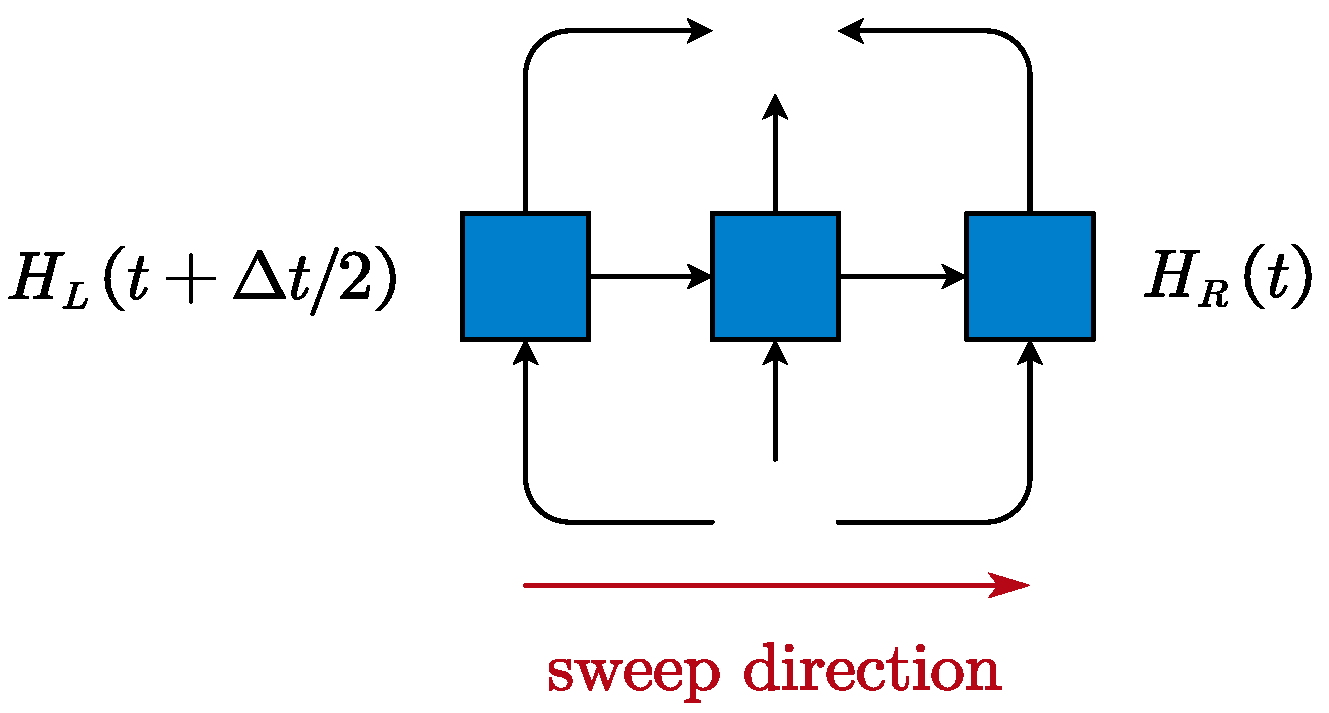
\includegraphics[height=0.2\linewidth]{images/effH1 t.pdf}}
				\subfigure{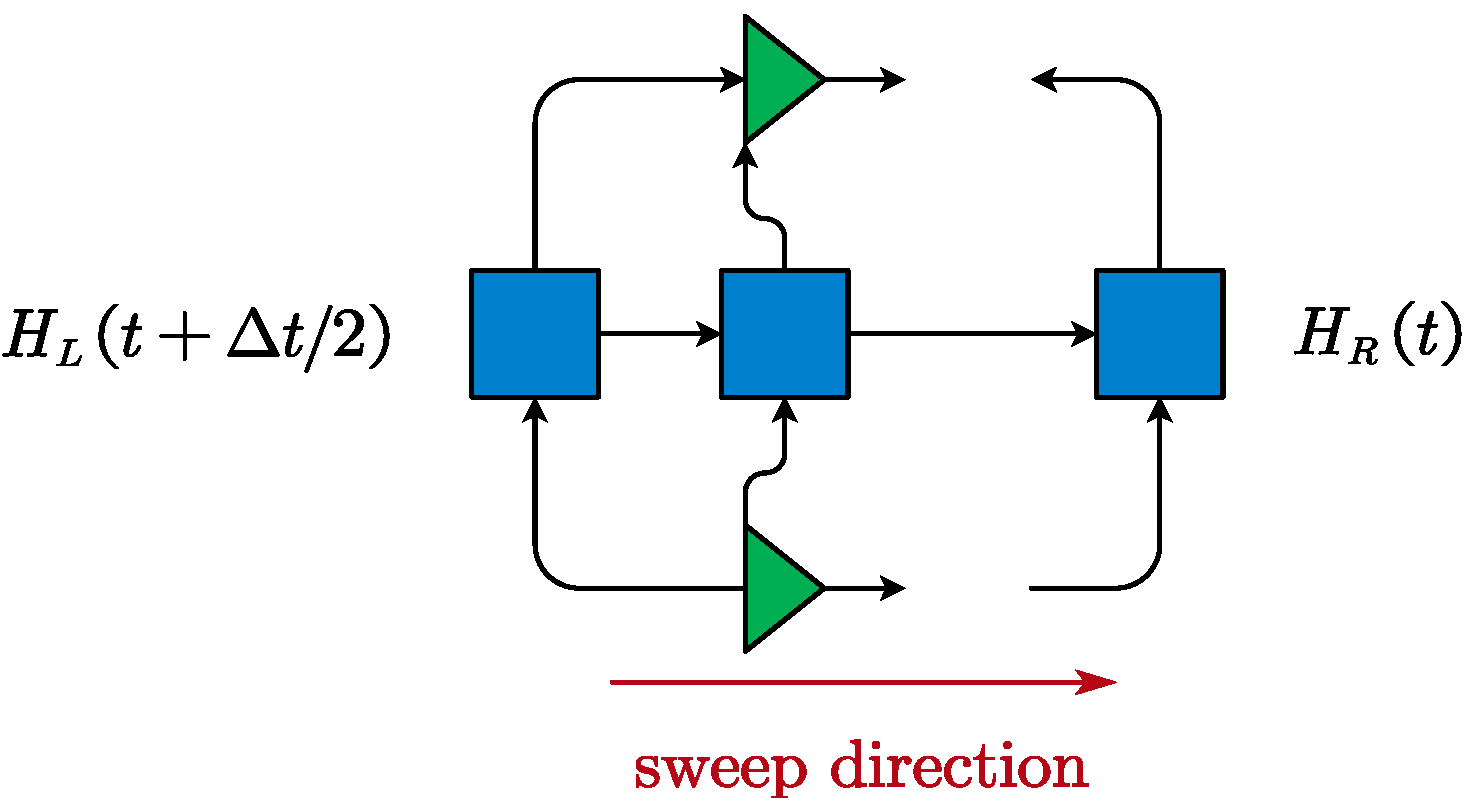
\includegraphics[height=0.21\linewidth]{images/effH0 t.pdf}}
			\end{figure}
		\end{itemize}
	\end{itemize}
\end{frame}

\begin{frame}
	\frametitle{TDVP: 2-site integration}
	Sweep schemes
	\begin{itemize}
		\item Calculate the left/right environment $H_L(t+\Delta t/2)/H_R(t)$.
		\begin{figure}[H]
			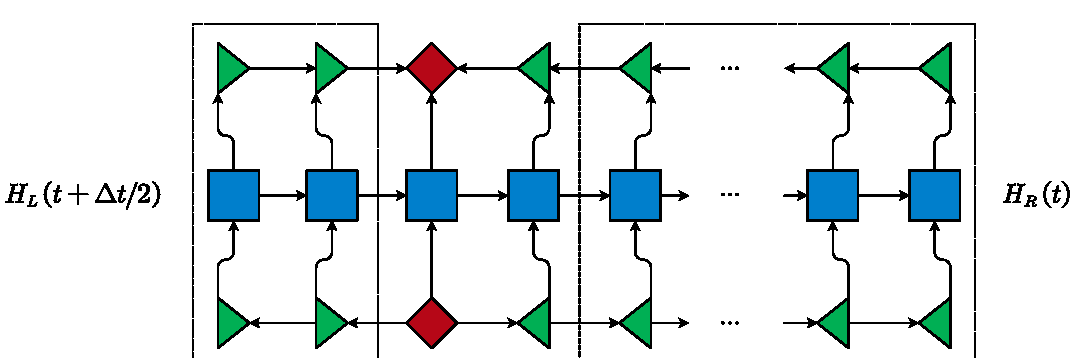
\includegraphics[width=0.8 \linewidth]{images/LRenv2 t.pdf}
		\end{figure}
	\end{itemize}
\end{frame}

\begin{frame}
	\frametitle{TDVP: 2-site integration}
	Sweep schemes
	\begin{itemize}
		\item Calculate the effective Hamiltonian $H_{eff}^{(2)}$
		\item Time evolution $A_iA_{i+1}(t+\Delta t/2) = \exp(-iH_{eff}^{(2)}\Delta t / 2)A_iA_{i+1}(t)$ 
		\item OrientSVD and calculate the center with inverse evolution $A_{i+1}(t) = \exp(iH_{eff}^{(1)}\Delta t /2) A_{i+1}(t+\Delta t/2)$, then regard it as nextsite.
		\begin{figure}[H]
			\centering
			\subfigbottomskip=2pt
			\subfigcapskip=-5pt
			\subfigure{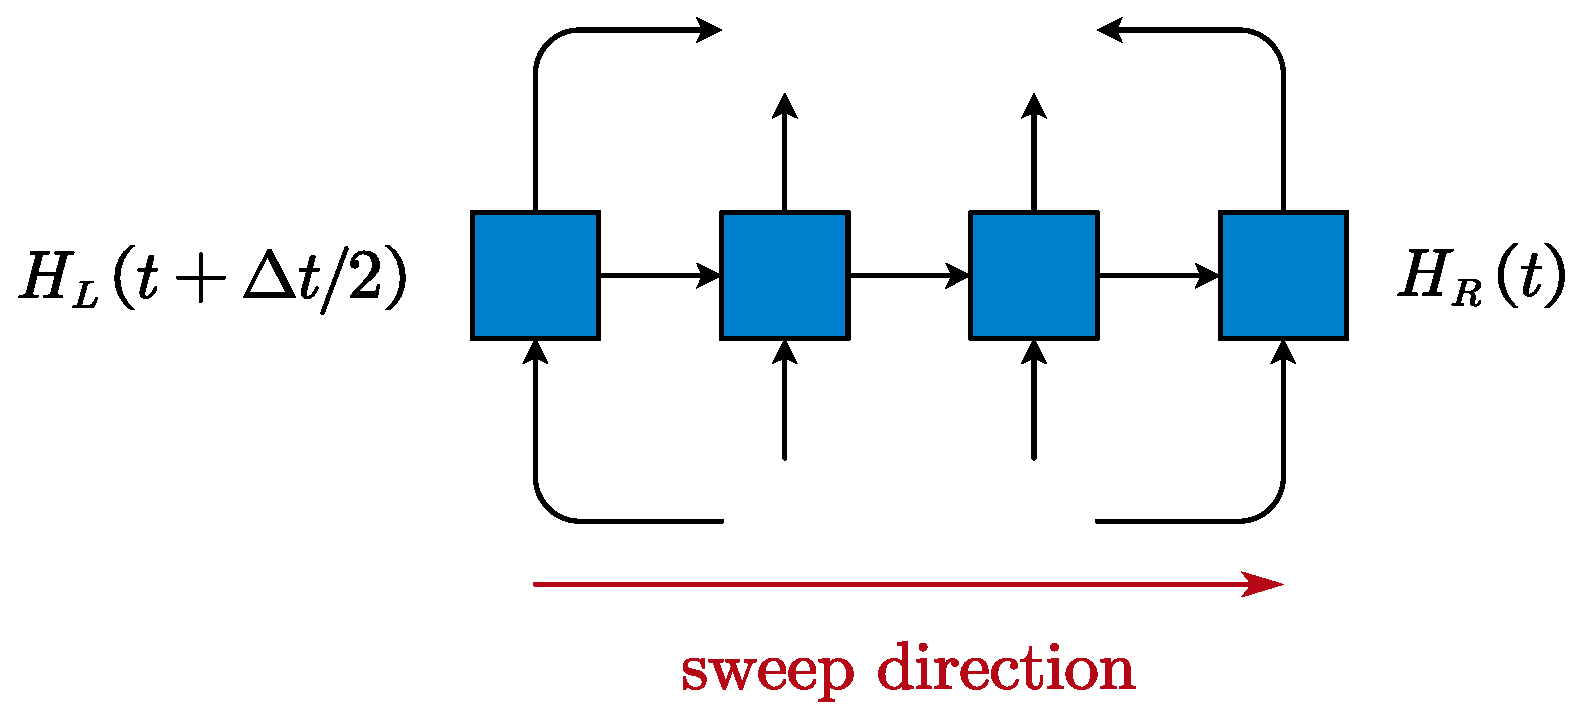
\includegraphics[height=0.2\linewidth]{images/effH2 t.pdf}}
			\subfigure{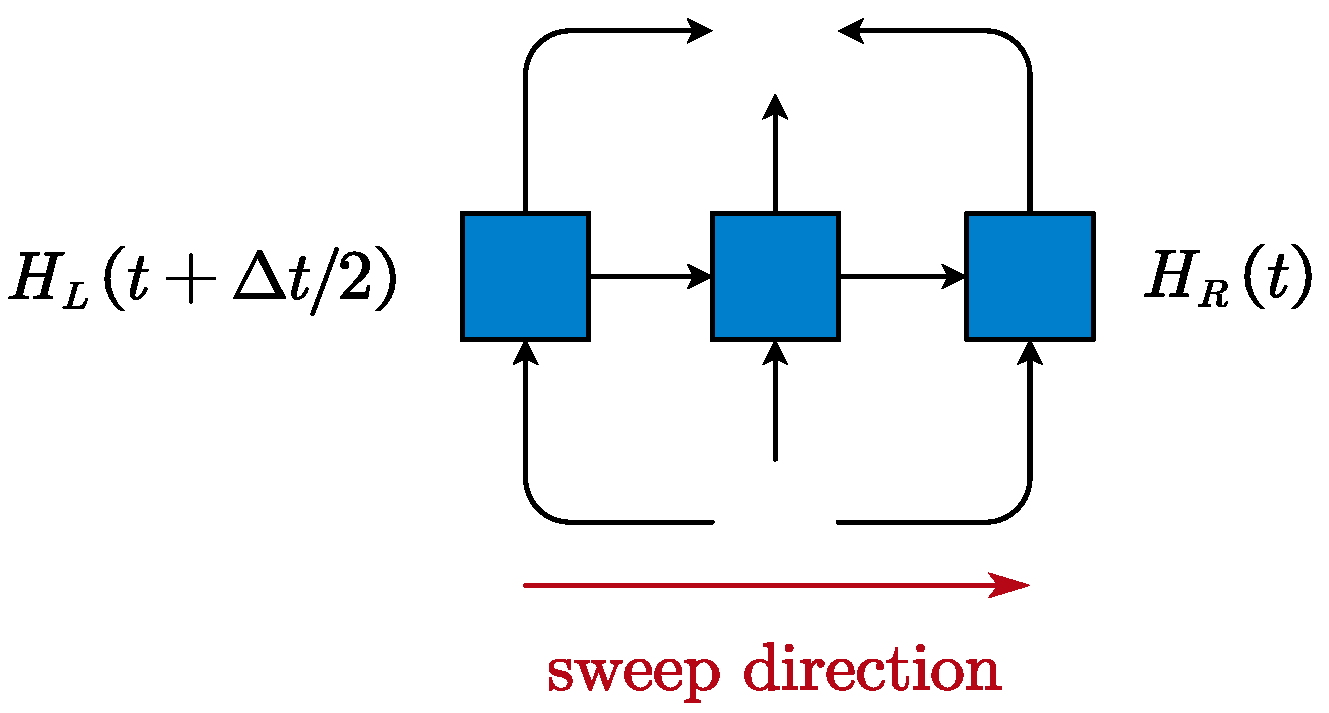
\includegraphics[height=0.2\linewidth]{images/effH1 t.pdf}}
		\end{figure}
	\end{itemize}
\end{frame}

\end{document}
